\section{Materials and Methods}

\subsection{Data Sets}

\subsubsection{Patient-Derived Cell Line (PDCL)}

This database has been established by the \acrlong{icm} (ICM, Paris).
Cells comes from tumour of 20 patients diagnosed with glioblastoma, they were then cultured \textit{in vitro} before RNA-Seq analysis was conducted.
Results include the raw count value of approximately 20,000 genes for each sample.
Only one replicate per sample is available.

Because the \acrshort{pdcl} dataset does not include matching control samples, we compared them to astrocytes RNA-Seq data from a study on the characterization of different astrocytic models by Lundin \textit{et al} \cite*{Lundin2018}.
The dataset contains 4 samples of different astrocyte cell lines with 3 replicates per sample, all information about the samples including the accession number are listed in table \ref*{table:list-control-samples}.

\begin{table}
    \centering
    \begin{tabular}{ |c|c| }
        \hline
        Accession Number & Sample name \\
        \hline
        GSM2927872 & AF22\_NES-Astro\_d29\_Br1 \\
        GSM2927873 & AF22\_NES-Astro\_d29\_Br2 \\
        GSM2927874 & AF22\_NES-Astro\_d29\_Br3 \\
        \hline
        GSM2927881 & iCellAstro\_Br1 \\
        GSM2927882 & iCellAstro\_Br2 \\
        GSM2927883 & iCellAstro\_Br3 \\
        \hline
        GSM2927884 & CCF\_Br1 \\
        GSM2927885 & CCF\_Br2 \\
        GSM2927886 & CCF\_Br3 \\
        \hline
        GSM2927887 & phaAstro\_Br1 \\ 
        GSM2927888 & phaAstro\_Br2 \\ 
        GSM2927889 & phaAstro\_Br3 \\ 
        \hline
    \end{tabular}
    \caption{
        List of samples with their accession number used as the control condition.
        Each sample can be either downloaded separately or as one raw count file in text format using the accession number GSE109001 on \acrfull{geo}.
        The accession number is an ID to retrieve date on the \acrshort{geo} database.
        The dataset contains 4 samples of different astrocyte cell lines with 3 replicates per sample.
        At the time of the publication, data were last updated on January 29, 2019.
    }
    \label{table:list-control-samples}
\end{table}

\subsubsection{The Cancer Genome Atlas (TCGA) }

The dysregulations found in this dataset were compared with glioblastoma data from the TCGA-GBM project available on the \acrshort{tcga} database (version 33.1, May 31 2022).
The TCGA-GBM project aim to sequence the mutations and gene expressions for the glioblastoma disease.
Glioblastoma tumour was the first to be sequence by the \acrshort{tcga} initiative.
The dataset contains gene expressions for primary/recurrent tumours and solid normal tissues.
All samples have been processed following the bioinformatic pipeline defined by \acrshort{tcga} and described on their website.
Few normal transcriptomes profiling are available for the brain, hence this dataset is over-represented by tumourous samples with 169 tumour samples and 5 control samples.

\subsection{Differential Expression Analysis}

This analysis consist of comparing the expression of genes in a tumour against a control to look for genes whose expressions are deregulated (over or under expressed).
This generate a list of genes as a result that is then used in the second step to perform pathways enrichment analysis.
Different portions of RNA, called reads, are sequenced during RNA-Seq experiment.
To quantify the expression of a gene, those reads are then mapped to the genes of a reference genome.
The number of mapped reads is computed for each gene giving a raw value called raw counts.
Factors such as transcript (mRNA that went through post-transcriptional modification) length, the total number of reads and sequencing biases can impact the raw counts value, therefore this value is normalized to obtain a value suitable for comparison \cite*{Conesa2016}.
Different tools are available to perform \acrshort{de} analysis such as edgeR \cite*{Robinson2010}, Limma \cite*{Ritchie2015}, DESeq2 \cite*{Love2014} and \acrshort{penda} \cite*{Richard2020}.
In this study, we selected DESeq2 \cite*{Love2014} and \acrfull{penda} to carry out the \acrshort{de} analysis.

\acrshort{de} analysis was performed on the two datasets \acrshort{pdcl} and \acrshort{tcga} where we compared all the tumourous samples against all the normal samples (glioblastoma versus normal).
With this approach, we identify a typical profile or the typical gene deregulations in the case of glioblastoma.
Glioblastomas are known to be heterogeneous tumours, hindering therapeutic success \cite*{Neftel2019,Delgado-Lopez2016, Quinones2018}.
Since the approach described does not account for heterogeneity between patients, we compared each sample one by one with all the controls for both datasets.
This second approach defines the deregulation for each sample, giving the ability to determine the biological functions that are frequently deregulated or cell line specific.
However, DESeq2 hypothesis assumes several replicates are available in the dataset.
This condition is not met since in this case we compare only one sample with no replicate against all the controls, leading to reduced accuracy.
Thus we will use \acrshort{penda}, a statistical method designed for this purpose.
Because this tool does not compute a metric to perform its test (rank comparison method) the results from \acrshort{penda} are then fed to G:Profiler only.

\subsubsection{DESeq2}

DESeq2 uses a negative binomial distribution (also called gamma-Poisson distribution) to model read counts and perform a Wald Test to test for differential expression \cite*{Love2014}.
As DESeq2 includes a built-in normalization method, only raw counts can be used as input to the tool.
It also performs an automated detection of outliers, detection of genes with low counts, estimation of model parameters and gene expression dispersion.
The $log_2$ fold change value is a numeric value used to quantify the strength and direction of deregulation (up or down) between a condition and the control.
We selected DESeq2 for the features cited above, its ease of use and its overall performance \cite*{Love2014}.
The Wald-Test statistic has 2 useful features : (1) the value is positive when a gene is upregulated and negative when it is downregulated; (2) the higher the absolute value of the statistic is, the more significant the fold change is, therefore it combines biological and statistical informations at the same time.

\subsubsection{ Personalized Differential Analysis (PenDA)}

\acrshort{penda} is a rank-based method to perform \acrshort{de} using a sample from the condition to test for differential expression and a reference dataset \cite*{Richard2020}.
In comparison, population-scale analysis tools like DESeq2 usually model the data using a distribution law and perform a statistical test to detect differential expression.
Those methods were designed to investigate typical gene deregulations patterns, consequently, they do not provide information at the individual scale.
They are also sensitive to batch effects and the choice of normalization applied.
With all these limitations in mind, \acrshort{penda} was designed to investigate gene expression data at the individual scale with robustness to batch and normalization effects.
For our PenDA analysis, we normalize the counts using the pseudo-count method ( $log_2(count + 1)$ ) from the DESeq2 package before filtering and ranking with the \acrshort{penda}.

\subsection{Pathway Enrichment Analysis}

Here, we use the list of deregulated genes identified by the \acrlong{de} analysis as input to investigate the deregulated pathways in the \acrshort{pdcl} and \acrshort{tcga}.
The \acrlong{pdcl} dataset was analyzed at both the population and the patient scale while the \acrshort{tcga} was only examined at the population scale.
Here we selected the two tools G:Profiler and \acrfull{gsea} to run the pathway enrichment analysis.
Both tools gives as an output a list of pathways with a p-value associated to each pathways.
The p-value represent the probability that a pathways is found enriched due to a random effect rather than truly due to the condition studied.
Therefore the lower the p-value is, the more significant the result.
When statistical testing is repeated, the p-value can be found significant by chance alone.
Multiple-testing correction method adjust the significance of the p-value to correct for this effect.
The most commonly used method, and the one used in this paper, is Benjaminini-Hochberg \acrfull{fdr} multiple-hypothesis correction method.
Like for the p-value, we want the \acrshort{fdr} to be the lowest possible, generally below 0.05 yet 0.1 is also found in the literature \cite*{Reimand2019}.
To reduce the number of pathways to investigate in the literature and to ensure the reliability of the result, we selected the results with a \acrshort{fdr} below 0.1 in both G:Profiler and \acrshort{gsea}.

\subsubsection{G:Profiler}
G:Profiler is a tool for finding biological processes enriched in a list of genes (for example a list of deregulated genes or a list of mutated genes) accessible either online using their web interface or using their API and libraries \cite*{Raudvere2019}.
Only the names of the genes are needed in input.
It searches for pathways or biological categories which are over-represented in a list of genes using the cumulative hypergeometric test.
G:Profiler includes multiple hypothesis correction methods with a built-in method called g:SCS, developed by the G:Profiler team, or the more known Bonferroni and \acrshort{fdr} correction method.
We choose the \acrshort{fdr} correction method as \acrshort{gsea} use the same method to be consistent between tools.

\subsubsection{Gene Set Enrichment Analysis (GSEA)}

\acrshort{gsea} is a rank-based method developed by Subramanian \textit{et al} \cite*{Subramanian2005} that determines the pathways enriched in a list of genes ordered by a metric.
This ranking metric is a float value that can be positive or negative, for example, the fold change in expression between a tumour and a control.
The list is sorted in decreasing order, thus genes the most strongly or significantly upregulated will be at the top of the list and at bottom for the downregulated.
The \acrshort{gsea} approach determines whether the genes involved in a gene set are mostly distributed at the top or the bottom of a gene list.
The algorithm of \acrshort{gsea} runs through the list of genes to compute a score called  \acrfull{es}, similar to a weighted Kolmogorov-Smirnov-like statistic.
A gene metric is added to the score if it is present in the pathways, substracted otherwise.
The score is then determined by the maximum deviation from zero.
The \acrshort{es} of a null distribution, generated by permutating the genes in the dataset or the phenotype of the samples, is computed using the same algorithm.
The score of the tested pathways is compared with the score of the null distribution to compute the significance of a result.
\acrshort{gsea} use the \acrshort{fdr} method to adjust for multiple hypothesis testing.
Despite both of them need a list of genes, G:Profiler needs only the genes symbol as input while for \acrshort{gsea}, each gene must be assigned a metric value.
A study from Zyla \textit{et al} has shown that the \acrshort{gsea} metric used can impact the results \cite*{Zyla2017}.
They evaluated the performance of 16 different metrics and found that the absolute value of the Moderated Welch Test statistic, the Minimum Significant Difference, the absolute value of the Signal to Noise ratio and the Baumgartner-Weiss-Schindler test statistic give the best outcome.
Most of the metrics tested are statistics computed during a test.
Wald-Test statistic combines both biological and statistical information, suggesting it is a valuable metric for running \acrshort{gsea} analysis.
Thus, we ranked the genes of the dataset with the statistic of the Wald-Test computed by DESeq2 before we run \acrshort{gsea}.

\subsubsection{Gene Matrix Transposed (GMT)}

Biological information must be provided to pathway enrichment tools as gene sets, a group of genes sharing a common biological feature (for example a biological function or chromosomal location).
Both G:Profiler and \acrshort{gsea} need a gene supplied in a tabular format called \acrfull{gmt} where each row is a gene set, in this study gene sets are pathways.
The first column of the file contains the pathway ID, the second column contains a description and the remaining column are all the genes involved in the pathway.
G:Profiler is updated regularly with the most common databases such as \acrshort{kegg}, Reactome, WikiPathways, miRTarBase, Gene Ontology, etc.
Except for a few databases due to licensing limitations, including \acrshort{kegg}, all built-in G:Profiler's gene sets can be downloaded from their website.
\acrshort{gsea} includes built-in gene sets from the Molecular Signatures Database (MSigDB) which can be downloaded.
G:Profiler and \acrshort{gsea} allow the user to submit custom \acrshort{gmt} files as well.
We downloaded gene sets from \acrshort{kegg} \cite*{Kanehisa2019} and Reactome \cite*{Gillespie2022}, two biological databases with curated sets of data.
It is recommended to use different databases as the same pathways can have different definitions among databases.
For example, the glycolysis is defined as \textit{canonical glycolysis} in Gene Ontology, \textit{glycolysis} in Reactome and \textit{Glycolysis/Gluconeogenesis} in \acrshort{kegg}.
It is beneficial to exclude small and large pathways as : (1) small pathways are redundant with larger pathways while large pathways are often too general (metabolism, cell-cycle); (2) small pathways are never picked up by pathway enrichment tools while large pathways tend to always shows-up in the results; (3) higher number of pathways in the data makes multiple-testing correction more strict \cite*{Reimand2019}.
Pathway sizes of 10-15 to 200-500 genes are recommended yet sizes of 2,000 genes can be found in the literature \cite*{Reimand2019}.
In this paper, we kept pathways of 15 to 500 genes.

\subsection{Implementation of the Workflow and Interpretation of the Results}

The protocol used in this study can be split into three steps :
\begin{enumerate}
    \item \acrfull{de} analysis is used to analyze RNA-Seq data, i.e. to produce a list of the genes that are deregulated in glioblastoma.
    We compared, gene expression between samples taken from a patient's tumour with healthy astrocyte cells.
    \item Pathway Enrichment allows to find the deregulated pathways in the list of genes defined in the \acrshort{de} analysis.
    Pathway enrichment analysis search for pathways that are enriched in a list of genes, in other words, pathways that are deregulated.
    For this step, we used two methods documented in the literature : G:Profiler and \acrfull{gsea}.
    We downloaded pathway information from \acrfull{kegg} and Reactome, two pathway database that defined biological processes of the cell.
    \item We compare the biological processes found deregulated in our datasets to identify the impaired mechanisms.
    In this regard, we mapped each pathway to their highest ancestors in the hierarchy of pathways to define biological categories for each database.
    For example, the entry \textit{G1/S phase transition} in Reactome is a child pathway of the entry \textit{Cell-Cycle}.
    Thus, we class this pathway in the Cell-Cycle category.
    To avoid false positives and reduce the number of pathways found, we only considered the pathways that are below the significance threshold in both G:Profiler and \acrshort{gsea} during the analysis of the results.
\end{enumerate}
All the data analyses were carried out with the R programming language.
G:Profiler pathway enrichment were performed with the official R librarie (version 0.2.1), and \acrshort{gsea} pathway enrichment with the \textit{fgsea} R package available on Bioconductor (version 1.12.0) \cite*{Korotkevich2021}.
Plots and reports, available as supplementary materials, were generated with the ggplot2 (version 3.3.6) and rmarkdown (version 2.14) R library.

\begin{figure}
    \centering
    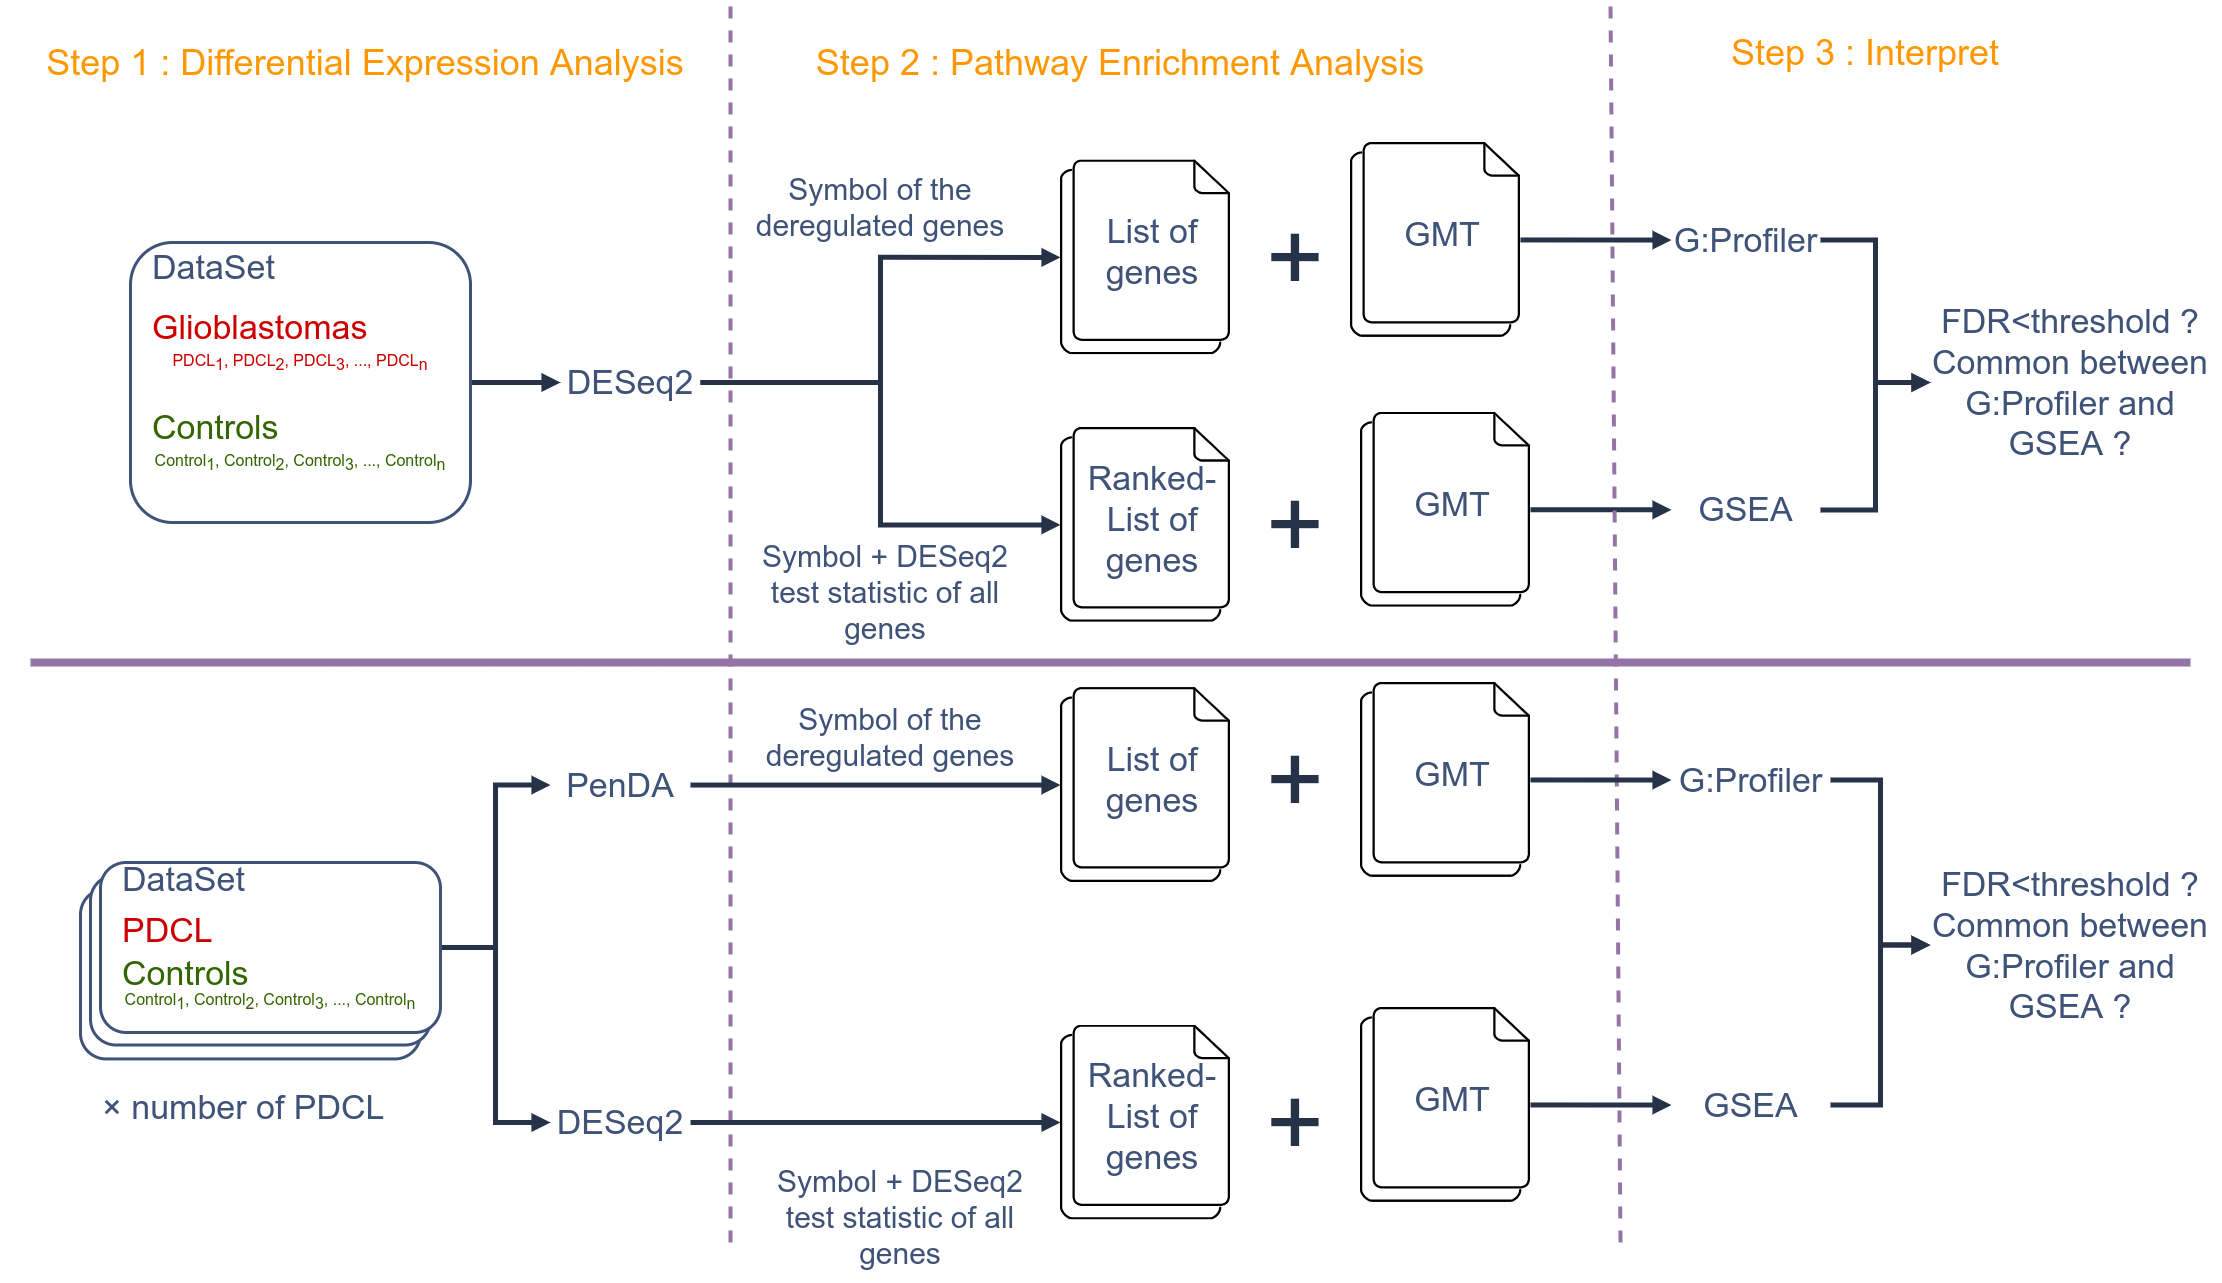
\includegraphics[width=\textwidth]{img/workflow-diagram}
    \caption{
        Diagram of the overall approach to search for the altered biological functions in glioblastoma.
        The top panel describes the workflow to find the typical deregulation in glioblastoma : a global analysis at the population level.
        In this case, we compare all the controls against all the glioblastoma samples in the dataset.
        We use DESeq2 to perform the \acrlong{de} analysis with each tumour and control samples considered as a "replicate of a typical patient or normal tissue".
        Then, we use G:Profiler and \acrshort{gsea} on the result of DESeq2 to perform pathway enrichment.
        The bottom panel describes the workflow adopted to assess the specific deregulations of each samples in both datasets : a personnalized analysis.
        Here we PenDA, a tool designed to perform \acrshort{de} analysis at the individual scale.
        In this case, we only apply G:Profiler on the PenDA results.
    }
    \label{fig:workflow-diagram-global}
\end{figure}

